\documentclass[10pt,pdf,hyperref={unicode}]{beamer}
\usepackage[utf8]{inputenc}
\usepackage[russian]{babel}

\usetheme{Berlin}
\setbeamertemplate{frametitle}[default][center]
\setbeamertemplate{footline}[frame number]

\title{Алгоритм Шеннона --- Фано}
\author{Сирота Александр}
\institute{\normalsize{ГУАП} \\ \scriptsize{5 факультет \\ Группа 5511}}
\date[3pt]{\scriptsize{Санкт-Петербург, 2016}}

\begin{document}
\begin{frame}
	\titlepage
\end{frame}

\begin{frame}
	\frametitle{План}

	\begin{enumerate}
		\item Основные сведения
		\begin{itemize}
			\item Коды переменной длины
			\item Префиксный код
			\item Пример префиксного кодирования
		\end{itemize}
		\item Основные этапы
		\item Построение кодового дерева
		\begin{itemize}
			\item Алгоритм
			\item Пример кодового дерева
		\end{itemize}
		\item Реализация
		\begin{itemize}
			\item Особенности
			\item Интерфейс
			\item Эффективность
		\end{itemize}
		\item Оценка сложности
	\end{enumerate}
\end{frame}

\begin{frame}
	\frametitle{Основные сведения}
	\textbf{Алгоритм Шеннона --- Фано} --- один из первых алгоритмов 
	сжатия, который сформулировали американские учёные Клод Шеннон и Роберт 
	Фано.
	\begin{itemize}
		\item Относится к вероятностным методам сжатия
		\item Алгоритм использует коды переменной длины
		\item Коды Шеннона --- Фано префиксные
	\end{itemize}
\end{frame}

\begin{frame}
	\frametitle{Коды переменной длины}
	При использовании \textbf{кодов переменной длины} символы кодируются набором бит различной длины.
	Часто встречающийся символ кодируется кодом меньшей длины, редко встречающийся --- кодом большей длины.
\end{frame}

\begin{frame}
	\frametitle{Префиксный код}
	\textbf{Префиксный код} (англ. prefix code) --- код, в котором никакое кодовое слово не является префиксом какого-то другого кодового слова.
\end{frame}

\begin{frame}
	\frametitle{Пример префиксного кодирования}
	$$
		U = \mathcal {f} a, b, c \mathcal {g}
	$$$$
		Z = \mathcal {f} 0, 1 \mathcal {g}
	$$$$
		c(a) = 00 \qquad
		c(b) = 01 \qquad
		c(c) = 1 \qquad
	$$

	Закодируем строку abacaba :
	$$
		c^*(abacaba) = 0001001000100
	$$

	Такой код можно однозначно разбить на слова:
	$$
		00\ 01\ 00\ 1\ 00\ 01\ 00
	$$
\end{frame}

\begin{frame}
	\frametitle{Алгоритм Фано: Основные этапы}
	Алгоритм Фано:
	\begin{enumerate}
		\item Выписать символы по убыванию вероятностей.
		\item Разделить список на две части с равными долями вероятности.
		\item Для первой части добавить к коду <<0>>, для второй --- <<1>>.
		\item Повторить шаги (1--3) для каждой части.
	\end{enumerate}
\end{frame}


\begin{frame}
	\frametitle{Алгоритм Фано: Этап 1}
	Символы первичного алфавита выписывают по убыванию вероятностей.
	\newline\newline
	\centerline{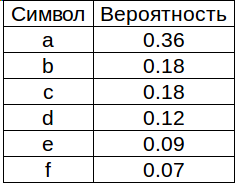
\includegraphics[height=8em]{alg0.png}}
\end{frame}

\begin{frame}
	\frametitle{Алгоритм Фано: Этап 2}
	Символы полученного алфавита делят на две части, суммарные вероятности символов которых максимально близки друг другу.
	\newline\newline
	\centerline{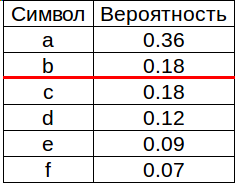
\includegraphics[height=8em]{alg1.png}}
\end{frame}

\begin{frame}
	\frametitle{Алгоритм Фано: Этап 3}
	В префиксном коде для первой части алфавита присваивается двоичная цифра «0», второй части — «1».
	\newline\newline
	\centerline{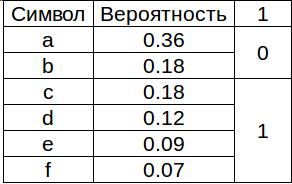
\includegraphics[height=8em]{alg2.png}}
\end{frame}

\begin{frame}
	\frametitle{Алгоритм Фано: Этап 4}
	Полученные части рекурсивно делятся и их частям назначаются соответствующие двоичные цифры в префиксном коде.
	\newline\newline
	\centerline{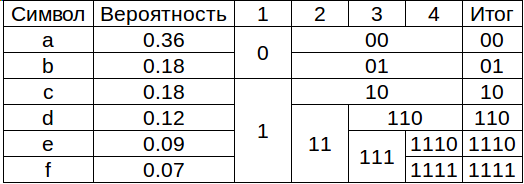
\includegraphics[height=8em]{alg3.png}}
\end{frame}

\begin{frame}
	\frametitle{Построение кодового дерева}
	Алгоритм:
	\begin{itemize}
		\item Код Шеннона — Фано строится с помощью бинарного дерева
		\item Всё множество кодируемых элементов соответствует корню дерева
		\item Множество разбивается на два подмножества с примерно одинаковыми суммарными вероятностями
		\item Если подмножество содержит единственный элемент, то такое подмножество последующему разбиению не подлежит
		\item Ветви кодового дерева размечаются символами 1 и 0
	\end{itemize}
\end{frame}

\begin{frame}
	\frametitle{Пример кодового дерева}
		
	\begin{figure}
		\begin{minipage}{0.25\textwidth}
		\raggedright{\scriptsize{Исходные символы:}}
		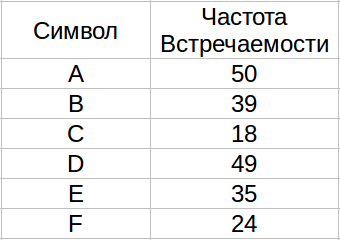
\includegraphics[width=\textwidth]{tree_sym.png}
		\end{minipage}
		\begin{minipage}{0.74\textwidth}
		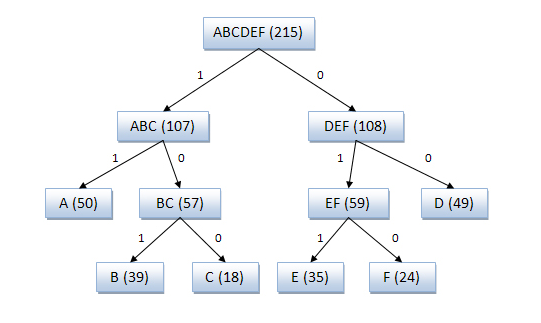
\includegraphics[width=\textwidth, trim= 20 20 50 15, clip=true]{tree.png}
		\end{minipage}
	\raggedright{Полученные коды:}
	\newline\newline
	\begin{minipage}[b]{\textwidth}
		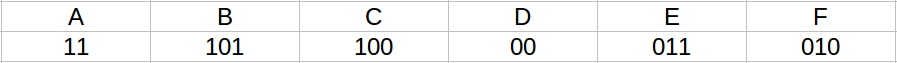
\includegraphics[width=\textwidth]{tree_code.png}
	\end{minipage}
	\end{figure}
\end{frame}

\begin{frame}
	\frametitle{Реализация}
	Особенности реализации:
	\begin{itemize}
		\item Простота
		\item Низкая сложность
		\item Иногда коды строятся неоптимально
		\item Необходимо дописывать шапку в файл
	\end{itemize}
\end{frame}

\begin{frame}
	\frametitle{Интерфейс}
	\begin{block}{Запуск программы}
		\$ ./fano <mode> <input> [ -o <output> ]
	\end{block}
	\begin{exampleblock}{<mode>}
		\textbf{'-e'} --- кодирование. Расширение входного файла \textbf{.txt}\\
		\textbf{'-d'} --- раскодирование. Расширение входного файла \textbf{.fano}
	\end{exampleblock}
	\begin{exampleblock}{<input>}
		Входной файл.
	\end{exampleblock}
	\begin{exampleblock}{<output>}
		Выходной файл. Если не указан, то будет 
		использовано имя входного файла + расширение.
	\end{exampleblock}
\end{frame}

\begin{frame}
	\frametitle{Пример сгенерированного словаря}
	Для фразы:
	\newline\newline
	\scriptsize{\textit{<<Lorem ipsum dolor sit amet, consectetur adipisicing elit. Odit sint cupiditate magni, illo officia facere magnam, ad pariatur ipsum explicabo sit nostrum aliquid nisi necessitatibus natus temporibus. Ut, optio, odit.>>}}
	\newline\newline
	\centerline{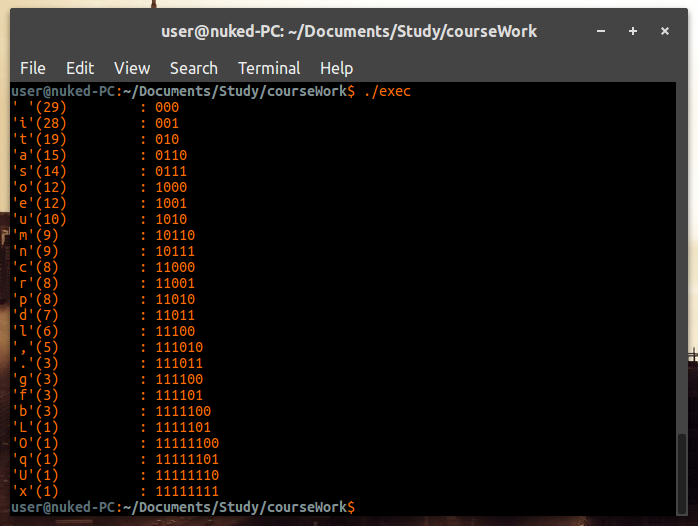
\includegraphics[height=20em]{gen.png}}
\end{frame}

\begin{frame}
	\frametitle{Эффективность}
		При сжатии текстового файла, содержащего один миллион слов~(7,6~Мб), 
		получился файл размером 4Мб. Эффективность сжатия - 47\%.\newline

		\centering
		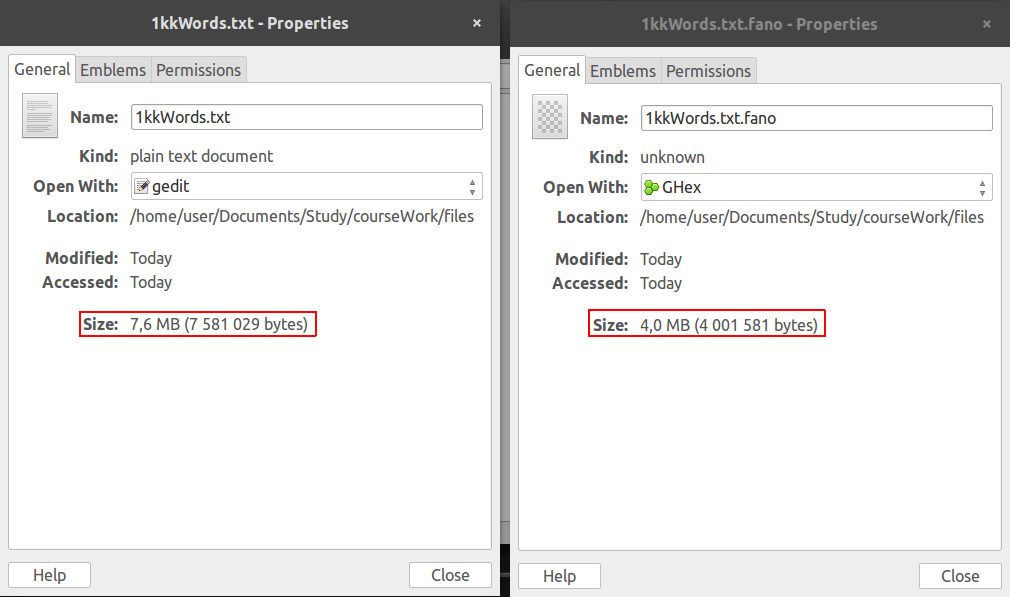
\includegraphics[width=0.8\textwidth]{compare.png}
\end{frame}

\begin{frame}
	\frametitle{Оценка сложности}
	Кодирование файла:\\ 
	\begin{itemize}
		\item Подсчёт символов: $O(n)$
		\item Построение дерева: $O(c)$
		\item Создание шапки для закодированного файла: $O(c)$
		\item Запись закодированных данных в файл: $O(n)$
	\end{itemize}
	Итоговая сложность --- линейная $O(n)$
\end{frame}

\begin{frame}
	\centerline{Спасибо за внимание!}
\end{frame}

\end{document}